% Chapter1
\chapter{Einleitung} \label{chapter:introduction}

% Inhalt
% Motiviert zum Thema und führt zum Thema hin.
% Erklärt wie man löst  
% Hintergrund und Ausgangspunkt (Heutzutage statische Systeme .. Dynamik… ) Wir wollen Methoden zur Verbesserung der Anlagen ausprobieren 
% Aufgabenstellung
% Leitfaden durch die Arbeit 		

% \section{Background and Motivation} 
% \section{Objectives of this Thesis}
% Ziel dieser Abschlussarbeit
% \section{Methodology for the Developement}  
% Methoden zur Entwicklung 
% \section{Thesis Outline}
% Abschlussarbeit Gliederung

% Mehr über die statische, hardgecodete SPS'n schreiben und die das bei Änderungen sehr viel neu  gecodet werden muss -> automatische Codegenerierung. 

% Heutzutage sind Produktionsanlagen so konstruiert, dass die Reihenfolge der einzelnen Fertigungszellen fest miteinander verkettet ist. Es herrscht eine unbewegliche, statische Folge der Stationen in dem jedes Anlagemodul autark arbeitet. Wenn es bei einem Teil zu einer Störung kommt, steht der ganze Produktionsfluss ausnahmslos. Zusätzlich ist die Flexibilität der Einsatzmöglichkeit einer Produktionsanlage eingeschränkt. Neue Module in die Verkettung hinzuzufügen erfordert enorme Umbauten und Kosten. \\\\
% Weiters kommt dazu, dass der Code auf der SPS neu programmiert werden muss, wenn ein Teil der Anlage anders verwendet werden soll. Dies hat einen Stillstand der Fabrik zur Folge. \cite{lb_SFC} Allgemein sind Produktionsanlagen sehr statisch gestaltet und können nur mit viel Aufwand geändert und angepasst werden. Bei Störungen kann nur schlecht reagiert werden was wiederum fatale Ausfälle in der Produktion nach sich zieht. \cite{wlepuschitz}

%Mithilfe von einem Modell, indem die Anlage abgebildet ist, und im weiteren Schritt einer Codegenerierung . Dadurch kann ein manueller Schritt, automatisiert und dadurch auch zeit gespart werden.

% Viele Produkte auf einmal
% Individuell 
% Kurzer Lebenszyklus
% Konfigurierbar
% Hohe Qualität
% Kurze Wechsel zwischen Produkten
% Geringer Umlaufbestand 
% kundenindividuelle Massenproduktion 

%QUELLE LEPUSCHITZ!!!
%The world of industrial manufacturing faces serious challenges due to the dynamics of the 21st century market. Even though the demand for mass commodities remains constant or even rises as a result of growing demand from emerging economies, the continuously decreasing life cycle span of products such as mobile phones combined with an increasing individualization significantly boosts the product variety [1]. In this context, manufacturing systems are required to support mass customization with the capability of “made-to-order” instead of “made-to-stock” [2]. The concept incorporates “the ability to provide individually designed products and services to every customer through high process agility, flexibility and integration” [3]. The principle of mass customization was anticipated by Alvin To✏er already in 1970 and detailed for the first time by Stan Davis in 1987 [4]. The automotive indus- try, once prototypical for mass production, was among the earlier adopters of mass customization around 1990 with Toyota o↵ering a five-day delivery for customers, who could decide from a range of modular options concerning their desired car [5]. Even though the possibilities and conceptual aspects were already described before the turn of the millenium, the importance of mass customization as a major manufacturing strategy in various domains ranging from the food industry to mobile phones emerged only during the last decade, thereby introducing new technological demands and challenges [6]. Put in a nutshell, production systems are forced to “produce a number of different, high-quality products via short production runs, short ch times, and low work-in-process” [5].
%Die Dynamik des heutigen Markts erfordert Produktionssysteme, die in der Lage sind eine große Produktvielfalt mit geringem Aufwand zu erzeugen, um rasch auf individuelle Kundenwüsche reagieren zu ko ̈nnen. Jedoch bie- ten die derzeit eingesetzten Produktionssysteme aufgrund ihres starren Aufbaus nicht genügend Flexibilität. Im Gegensatz dazu sind rekonfigurierbare Produktionssysteme aus modularen Komponenten aufgebaut, welche flexibel modifiziert beziehungsweise je nach beno ̈tigter Funktionalita ̈t dem System hinzugefu ̈gt oder aus dem System entfernt werden ko ̈nnen. Entsprechende Software-Konzepte sind daher fu ̈r die Beherrschbarkeit und Steuerbarkeit solch eines verteilten Systems notwendig.
%______________________________
%URSPRÜNGLICHE EINLEITUNG
%Produktionssysteme im 21. Jahrhundert müssen wachsenden Anforderungen gerecht werden. Besonders die auftragsbezogene Einzelproduktion bringt große Herausforderung mit sich. Dabei wird eine kurze Durchlaufzeit bei hoher Qualität ebenso erwartet, sowie keine oder nur geringe Mehrkosten gegenüber der herkömmlichen Serien- und Massenproduktion. Eine Produktionsanlage muss daher unterschiedliche, hoch konfigurierbare, Produkte auf einmal schaffen können. Zusätzlich haben sich Lebenszyklen von Waren verringert, welches ein schnelles umstellen der Produktionssysteme fordert.\cite{wlepuschitz_2014} \\

Der Bereich der industriellen Fertigung muss im 21. Jahrhundert wachsenden Anforderungen gerecht werden. Die Dynamik des Marktes erfordert eine konfigurierbare Massenproduktion, die es erlaubt auf individuelle Kundenwünsche einzugehen. Es wird von Produktionssystemen erwartet, dass sie "`made-to-order"' anstatt von "`made-to-stock"' Waren erzeugen können. Besonders die auftragsbezogene Einzelproduktion bringt große Herausforderung mit sich. Dabei wird eine kurze Durchlaufzeit bei hoher Qualität ebenso erwartet, wie keine oder nur geringe Mehrkosten gegenüber der herkömmlichen Serien- und Massenproduktion. Zusätzlich verringern sich laufend die Lebenszyklen von Waren, die wiederum eines flexibleren Produktionssystems bedürfen. Diese sind heutzutage allerdings wegen ihres starren Aufbaus oft nicht im Stande diese Anforderungen zu erfüllen. \cite{wlepuschitz_2014} \\\\
Diese Anpassungsfähigkeit fordert ein schnelles Umstellen von Produktionssystemen. Hingegen ist es vielfach so, dass bei Änderungen wie dem Hinzufügen oder Entfernen von Teilen großer Aufwand nötig ist, um das System in neuer Zusammensetzung in Betrieb zu setzen. Besonders für die Steuereinheiten von Produktionsanlagen, die sog. speicherprogrammierbare Steuerung (SPS), muss ein Großteil des Programm-Codes neu implementiert werden. \cite{Lepuschitz_PhaseAgent}  
Das Diplomprojekt hat sich zur Aufgabe gemacht, diesen Implementierungsschritt zu untersuchen und zu klären, in welchem Ausmaß und in welcher Art und Weise sich dieser Schritt anhand einer Implementierung auf einer Laboranlage automatisieren lässt. 
 Diese Problematik der Automatisierung wird in den nächsten Abschnitten weiter beleuchtet. Dabei wird auf Motivation und Hintergrund der Arbeit eingegangen und der Stand der bereits realisierten Projekte erläutert. Ein Überblick über die Aufgabenstellung sowie ein Leitfaden durch die Arbeit schließen dieses Kapitel ab. 
\section{Hintergrund und Ausgangspunkt}
Der Verein Practical Robotics Institute Austria, kurz PRIA, dient der Förderung des wissenschaftlich-technischen Nachwuchses durch Robotik und nimmt sich der Forschungsaufgaben in verwandten Fachgebieten der Robotik und Automation an.
Im Rahmen diese Instituts wird in dem Projekt „Batch Process Automation with an On\-to\-lo\-gy-driven Multi-Agent System (BatMAS)“ an einem ontologiebasierten Informationsmodell geforscht. Dadurch sollen die Konzepte von Produktionssystemen  beschrieben werden. BatMAS wird von  der österreichischen Forschungsföderungsgesellschaft (FFG) unterstützt. Dabei sollen intelligente Softwarekomponenten (Agenten) eingesetzt werden, die Aufträge dynamisch zuteilen um die Produktionsdauer zu verringern und damit den Durchsatz des Systems zu erhöhen.\\\\
Das Projekt Batch\_it greift diese Ansätze auf und hat sich zum Ziel gesetzt eine modellbasierte Entwicklung der Steuerung einer Produktionsanlage umzusetzen. Hierfür wird in einem Modell eine Produktionsanlage abgebildet, um eine automatische Codegenerierung basierend auf Modell zu ermöglichen. Wenn es zu Änderungen der Produktionsanlage kommt, können diese im Modell angepasst werden und durch einen Codegenerierung der nötige Anpassungsschritt der Implementierung der SPS automatisiert werden.
\begin{figure}[h!]
		\centering
		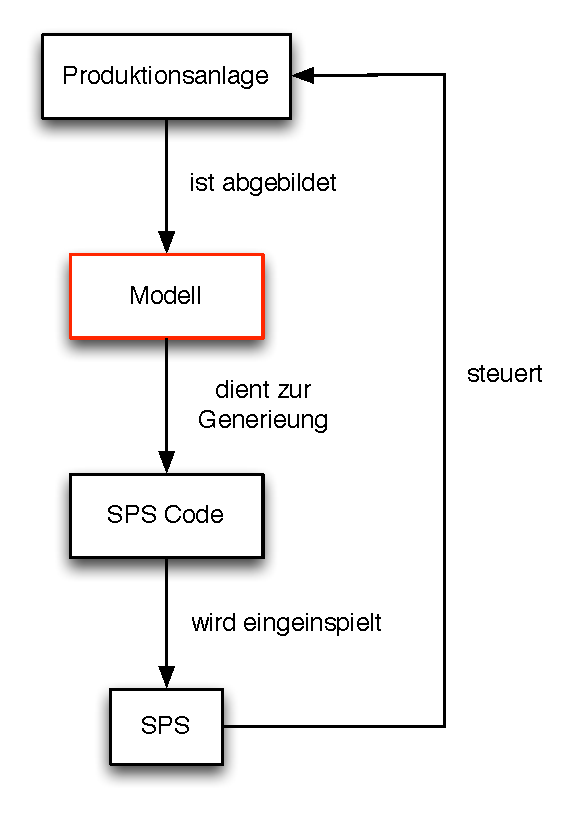
\includegraphics[width=0.37\textwidth]{graphics/konzept/konzept.pdf}
		\caption{Konzept für die modellbasierte Entwicklung der Steuerung}
		\label{fig:konzept}
\end{figure} \\
In der Abbildung~\ref{fig:konzept} ist zu sehen, dass die Produktionsanlage in einem Modell abgebildet ist. Aus diesem wird der SPS Code generiert und im weiteren Schritt in die SPS eingespielt. Daraufhin kann die Produktionsanlage gesteuert werden. 
%HSteuerungsaktivitäten und -funktionen, die es ermöglichen, endliche Mengen von Einsatzstoffen zu verarbeiten, indem diese unter Nutzung einer oder mehrerer Einrichtungen innerhalb eines endlichen Zeitraums einer geordneten

%Wir werden uns auf ist eine Norm für die chargenorientierte Fahrweise (Batch Control), die häufig als S88 oder SP88 bezeichnet wird. Sie ist eine Designphilosophie für Software, Ausrüstung und den Verfahrensablauf. 	

\section{Aufgabenstellung}
 Im Rahmen des Projekts Batch\_it soll eine Visualisierung und Steuerung sowie eine modellbasierte Entwicklung der Steuerung für eine Laboranlage für Chargenprozesse, die sich durch eine chargenorientierte Fahrweise (Batch Control) kennzeichnet,  implementiert werden. Dies umfasst das Erstellen von Prozeduren nach dem IEC 61512 Standard. Hierbei handelt es sich um Funktionen wie z.B. das Pumpen von Flüssigkeiten von Tank zu Reaktor oder das Heizen bzw. das Vermengen einer Flüssigkeit. Darüber hinaus werden daraus Rezepte nach dem IEC 61512 Standard entwickelt. Zusätzlich werden Fehlerszenarien einer Produktionsanlage aufgestellt, die zur späteren Entwicklung einer Fehleranalyse dienen.\todo{Satz ändern}Im weiteren Schritt wird eine Ontologie, welche das Modell darstellt, für die Abbildung der Anlage erstellt. Anhand dieser wird eine automatische Codegenerierung für die Steuerung der Anlage implementiert.

\section{Leitfaden durch die Arbeit}
TODO
